\documentclass[a4paper,10pt]{report}\input{../0.Préambule/Préambule_cours_prof}\begin{document}

\newpage
\section*{Pyramides et cônes 2}
\addcontentsline{toc}{section}{Pyramides et cônes 2}

\vspace{-3mm}
\begin{exer1}
Complète :

\begin{enumerate}[font=\color{exer1}]
\renewcommand{\arraystretch}{0.8}
\begin{tabularx}{\linewidth}{*{3}{>{\arraybackslash}X}}
\item $5,4$ m = \dots ~\dots ~\dots cm & 
\item $\np{3 263}$ m = \dots ~\dots ~\dots km & 
\item $14,7$ m$^2$ = \dots ~\dots ~\dots cm$^2$ \\ 
\item $\np{254 320}$ m$^2$ = \dots ~\dots ~\dots hm$^2$ & 
\item $5,68$ L = \dots ~\dots ~\dots mL & 
\item $\np{230 000}$ cm$^3$ = \dots ~\dots~\dots m$^3$ \\ 
\item $504,2$ cL = \dots ~\dots ~\dots L & 
\item $6,3$ dm$^3$ = \dots ~\dots ~\dots m$^3$ & 
\item $\np{5 362}$ dm$^3$ = \dots ~\dots ~\dots cm$^3$ \\ 
\item $0,07$ m$^3$ = \dots ~\dots ~\dots dm$^3$ & 
\item $\np{2 500}$ cm$^3$ = \dots ~\dots ~\dots L & 
\item $9,1$ cL = \dots ~\dots ~\dots cm$^3$ \\
\end{tabularx}
\end{enumerate}
\end{exer1}

\begin{exer1}

\medskip
\begin{enumerate}[font=\color{exer1}]
\item Calcule le volume d'une pyramide $SABCD$, de hauteur $6,3$cm et de base rectangulaire $ABCD$ telle que $AB=4,2$cm et $BC=3,5$cm. Donne le résultat en cm$^3$ puis en mm$^3$.

\item Calcule le volume d'une pyramide $MATH$, de base $ATH$ rectangle isocèle en $A$, de hauteur $[MA]$ et telle que $AT=3$cm et $MA= 4$cm.
\end{enumerate}
\end{exer1}

\begin{exer2}

\vspace{-2mm}\hspace{1.8cm}Pour construire la pyramide de Khéops, les égyptiens ont utilisé un volume d'environ $\np{2 643 000}$m$^3$ de pierres. La hauteur de la pyramide est de $146$m. Calcule le côté du carré constituant la base de la pyramide. Arrondis ton résultat au mètre.
\end{exer2}

\begin{exer2}
La société Truc fabrique des enseignes publicitaires composées de deux cônes de révolution de même diamètre $24$cm et de même hauteur $40$cm.

\noindent \begin{minipage}{6.5cm}
\begin{center}

\includegraphics[scale=0.5]{../40.Image/Exo_Pyramide_et_cone_3.png}
\end{center}
\end{minipage}
\begin{minipage}{9.5cm}
\begin{enumerate}[font=\color{exer2}]
\item Calculer le volume d'une enseigne. En donner la valeur exacte puis la valeur arrondie au dm$^3$.
\item Pour le transport, chaque enseigne est rangée dans un étui en carton ayant la forme d'un cylindre le plus petit possible et ayant la même base que les cônes.

\medskip
\noindent Calculer le volume de cet étui en négligeant l'épaisseur du carton. En donner la valeur exacte en cm$^3$ puis la valeur arrondie au dm$^3$.
\end{enumerate}
\end{minipage}
\end{exer2}

\begin{exer2}
On considère le cube ABCDEFGH de coté $5$cm.

\vspace{-8mm}
\noindent \begin{minipage}{9cm}

\vspace{5mm}
\begin{enumerate}[font=\color{exer2}]
\item Calcule le volume de cette pyramide, arrondi au cm$^3$.
\item Calcule les longueurs $AH$, $DG$ et $AG$ au millimètres près.
\item Calcule la mesure, arrondie au degré, de l'angle $\widehat{AHD}$.
\item Construis un patron de cette pyramide.
\end{enumerate}
\end{minipage}
\begin{minipage}{7cm}
\begin{center}
\begin{tikzpicture}[general,scale=0.5]
\draw(1,1.5) node[below] (A){$A$};
\draw(5,1) node[below] (B){$B$};
\draw(7,2) node[right] (C){$C$};
\draw(3,2.5) node[above left] (D){$D$};
\draw (1,5.5) node[left] (E){$E$};
\draw(5,5) node[above] (F){$F$};
\draw(7,6) node[right] (G){$G$};
\draw(3,6.5) node[above] (H){$H$};
\fill [color=exer2!20](A.north)--(H.south)--(G.west);
\fill [color=exer2!20](A.north)--(G.west)--(C.west);
\draw(3,2.5) node[above left] {$D$};
\draw [color=red, dashed] (A.north) -- (H.south);
\draw [color=red, dashed] (A.north) -- (C.west);
\draw [color=red, dashed] (A.north) -- (G.west);
\draw (1,1.5)-- (5,1)-- (5,5)--(1,5.5)--cycle;
\draw (1,5.5)--(3,6.5)--(7,6)--(5,5);
\draw (7,6)--(7,2)--(5,1)--(5,5);
\draw [dashed] (7,2)--(3,2.5);
\draw [color=red, dashed] (3,2.5)-- (1,1.5);
\draw [dashed] (3,2.5)-- (3,6.5);
\draw (1,5.5)--(5,5)--(7,6);
\end{tikzpicture}
\end{center}
\end{minipage}
\end{exer2}

\vspace{-3mm}
\begin{exer2}

\vspace{-2mm}\hspace{1.8cm}La pyramide régulière à base carrée $SABCD$ \\ci-dessous a une base de $50$cm$^2$ et une arête $[SA]$ de $13$cm.

\vspace{-10mm}
\noindent \begin{minipage}{11cm}

\vspace{8mm}
\begin{enumerate}[font=\color{exer2}]
\item Calculer la valeur exacte de $AB$ puis démontrer que : $AC=10$cm.
\item Soit $H$ le centre de $ABCD$. On admet que $(SH)$ est perpendiculaire à $(AC)$. Démontrer que $SH=12$cm puis calculer le volume de $SABCD$.
\end{enumerate}
\end{minipage}
\hspace{7mm}
\begin{minipage}{5cm}
\begin{flushright}
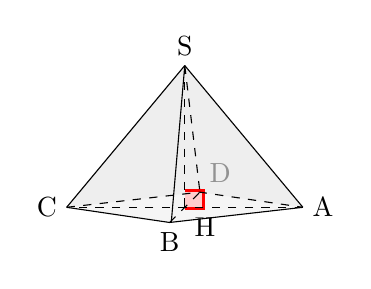
\begin{tikzpicture}[x=3cm,y=1.8cm,scale=0.5]
\tikzstyle{conefill} = [fill=gray!20,fill opacity=0.4] %couleur de fond
   
%coordonnées des sommets
\draw(0,2,0)node[above](S){S};
\draw(1,0,0)node[right](A){A};
\draw(-1,0,0)node[left](C){C};
\draw(0,0,1)node[below](B){B};
\draw(0,0,-1)node[above right](D){D};
\draw(0,0,0)node[below right](H){H};
   
%remplir les faces
\fill[conefill] (1,0,0)--(0,0,1)--(1,0,0)--(0,0,-1)--cycle; %base
\fill[conefill] (0,2,0)--(-1,0,0)--(0,0,-1); %arrière gauche
\fill[conefill] (0,2,0)--(-1,0,0)--(0,0,1); %avant gauche
\fill[conefill] (0,2,0)--(0,0,1)--(1,0,0); %avant droit
\fill[conefill] (0,2,0)--(1,0,0)--(0,0,-1); %arrière droit

\draw [line width=2pt,color=red] (0,0,0)--(0.15,0,0)--(0.15,0.22,0)--(0,0.22,0);
\fill[color=red!20] (0,0,0)--(0.15,0,0)--(0.15,0.22,0)--(0,0.22,0);

%tracer les arêtes
\draw (A.west)--(B.north)--(C.east);
\draw[dashed] (C.east)--(D.south west)--(A.west);
\draw (S.south)--(A.west);
\draw (S.south)--(C.east);
\draw (S.south)--(B);
\draw[dashed] (S.south)--(D.south west);
   
\draw [dashed] (S)--(0,0,0);
\draw[dashed] (A)--(C);
\draw[dashed] (B.north)--(D.south west);  
\end{tikzpicture}
\end{flushright}
\end{minipage}
\end{exer2}

\vspace{-3mm}
\begin{exer2}
La figure ci-dessous représente un cône de révolution $\mathcal{C}$ de hauteur $SO=20$cm et de base le cercle de rayon $OA=15$cm.

\noindent \begin{minipage}{12cm}
\begin{enumerate}[font=\color{exer2}]
\item Calculer en cm$^3$ le volume de $\mathcal{C}$, on donnera la valeur exacte sous la forme $k \pi$, $k$ étant un nombre entier.
\item Montrer que $SA=25$cm.
\item L'aire latérale d'un cône de révolution est donnée par la formule $\pi \times R \times SA$. ($R$ désignant le rayon du cercle de base). Calculer en cm$^2$ l'aire latérale de $\mathcal{C}$.

\noindent On donnera une valeur exacte sous la forme $n\pi$ ($n$ étant un nombre entier) puis une valeur approchée à $10^{-1}$ près.
\end{enumerate}
\end{minipage}
\begin{minipage}{5.2cm}
\begin{center}
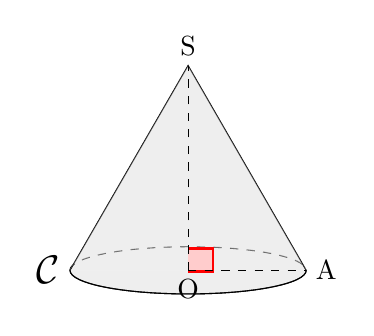
\begin{tikzpicture}[x=1.5cm,y=1.3cm,z={(0cm,-0.3cm)},scale=1]
\tikzstyle{conefill} = [fill=gray!20,fill opacity=0.4] %couleur de fond
%base inférieure
\filldraw[conefill] (-1,0,0) .. controls (-1,0,0.555) and (-0.555,0,1) .. (0,0,1) .. controls (0.555,0,1) and (1,0,0.555) .. (1,0,0);
\fill[conefill](-1,0,0) .. controls (-1,0,-0.555) and (-0.555,0,-1) .. (0,0,-1) .. controls (0.555,0,-1) and (1,0,-0.555) .. (1,0,0);
\draw[dashed] (-1,0,0) .. controls (-1,0,-0.555) and (-0.555,0,-1) .. (0,0,-1) .. controls (0.555,0,-1) and (1,0,-0.555) .. (1,0,0);
%remplir les faces latérales
\filldraw[conefill] (-1,0,0) .. controls (-1,0,0.555) and (-0.555,0,1) .. (0,0,1) .. controls (0.555,0,1) and (1,0,0.555) .. (1,0,0)--(0,2,0)--cycle;
\fill[conefill](-1,0,0) .. controls (-1,0,-0.555) and (-0.555,0,-1) .. (0,0,-1) .. controls (0.555,0,-1) and (1,0,-0.555) .. (1,0,0)--(0,2,0)--cycle;
\draw [line width=2pt,color=red] (0,0,0)--(0.2,0,0)--(0.2,0.2,0)--(0,0.2,0);
\fill[color=red!20] (0,0,0)--(0.2,0,0)--(0.2,0.2,0)--(0,0.2,0);
%diametre et hauteur
\draw[dashed] (0,0,0)--(1,0,0);
\draw[dashed] (0,0,0)--(0,2,0);
\draw(0,2,0)node[above](S){S};
\draw(0,0,0)node[below](O){O};
\draw(1,0,0)node[right](A){A};
\draw(-1,0,0)node[left]{\Large{$\mathcal{C}$}};
\end{tikzpicture}
\end{center}
\end{minipage}
\end{exer2}

\end{document}